
\section{Meshing}
\subsubsection{Editing the electrical mesh/layers}
The device structure is split up into layers of different materials.  These can be configured in layer editor.  Some of these layers will have the layer type 'active'.  An 'active' layer is a layer over which the electrical model will be applied.  The electrical model needs a finite difference mesh to to be setup for it to work.  Usually, this will be take care of automatically, by gpvdm.  However, some users will want fine control over the mesh.  The electrical mesh editor is depicted in figure \ref{fig:emesh}.


The buttons marked 1D, 2D and 3D at the top of the window can be used to toggle the simulation between 1D, 2D and 3D modes.  (Note, if you want to do 2D or 3D simulations you are best off using a default 2D simulation, such as the OFET simulation.  This is because to do 2D/3D simulations, a special newton solver configuration will be needed.) The table on the left hand side is used to configure the mesh.  The sum of the mesh layer thicknesses must exactly match that of the sum of the active layers.  If this is not the case, the model will automatically rewrite the electrical mesh, to something that has the correct dimensions but may not be what the user desires.  Automatic mesh configuration can be turned off though the cog icon.  The columns thickness and mesh points, determine the thickness of the mesh layer and the number of points on the mesh layer, if there is a uniform spacing between mesh points.  The column, 'step multiply' by how much to grow each step.  In this example, the mesh spacing is increased by a factor of 0.1 each step.  The toggle button left/right, defines on which side the mesh layer is generated.  In this example there are two mesh layers, one starting on the left and one starting on the right.  The resulting mesh is plotted in the graph at the bottom of the window.  It can be seen that a non-linear mesh has been generated.

\begin{figure}[ht!]
\centering
\includegraphics[width=\textwidth]{./images/emesh.png}
\caption{The electrical mesh editor}
\label{fig:emesh}
\end{figure}

\begin{figure}[ht!]
\centering
\includegraphics[width=\textwidth]{./images/mesh.png}
\caption{A 1D diagram of the mesh}
\label{fig:emeshdiagram}
\end{figure}


\subsubsection{Editing the optical mesh/layers}
The optical mesh automatically extends to cover the optical simulation window, so one does not usually need to worry about configuring it.  The optical material layers are defined in the list at the bottom of figure \ref{fig:emesh}.  The first column is a unique identifier, it must start with a hash symbol, but apart from that you can call it what you want.  The second column is the thickness of the layer.  The forth column is the material system, data files describing the material system are stored in the 'phys' directory.  Finally, the forth column tells the model if the layer is part of the active layer or not (more about that in the next section.)

\begin{figure}[ht!]
\centering
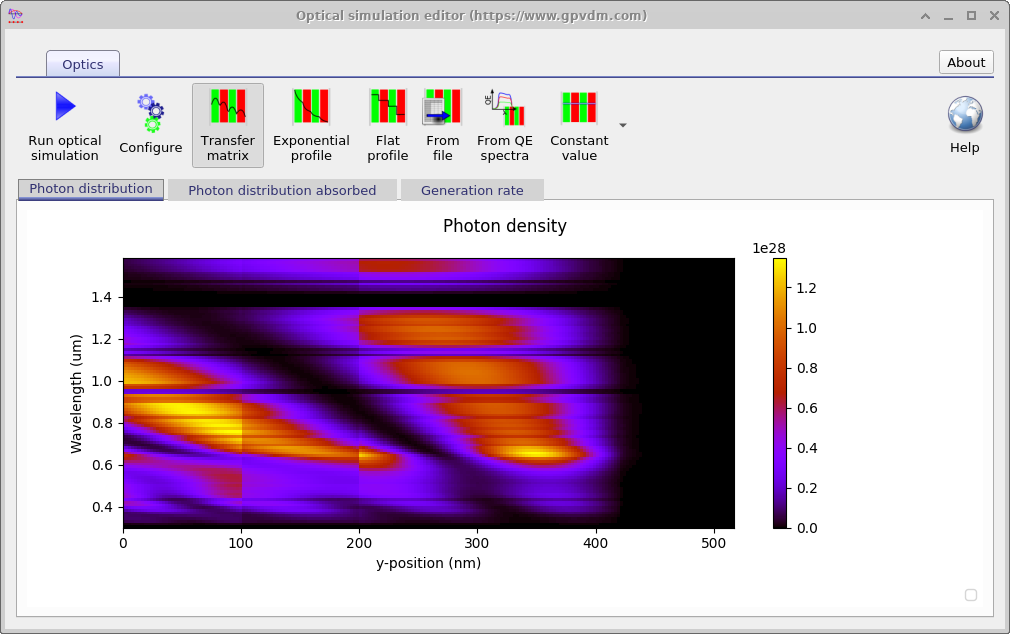
\includegraphics[width=\textwidth]{./images/opticalsimulation.png}
\caption{The electrical mesh editor}
\label{fig:opticalsimulation}
\end{figure}

\subsubsection{Interfacing the electrical and optical models}
In gpvdm there is both an electrical model and an optical model.  The optical simulation usually includes the glass substrate, the contacts and layers such as PEDOT:PSS.  The electrical simulation usually only covers the active layer of the device, thus a typically optical simulation is much bigger than the electrical simulation window.  The optical model feeds the calculated optical profile of the light into the electrical simulation.  You must therefore tell the optical model which layer in the optical simulation represents the active layer.  This is done by placing a 'yes' in the column 'Active layer' in figure \ref{fig:opticalsimulation}.
\newpage
\vfill
